\documentclass[11pt,a4paper,twocolumn]{article}
\usepackage[a4paper, top=2.2cm, bottom=2.2cm, left=1.8cm, right=1.8cm, columnsep=0.6cm]{geometry}
\usepackage[T1]{fontenc}
\usepackage[utf8]{inputenc}
\usepackage{lmodern}
\usepackage{amsmath,amssymb,amsfonts,amsthm}
\usepackage{booktabs}
\usepackage{algorithm}
\usepackage{algorithmic}
\usepackage{caption}
\usepackage{subcaption}
\usepackage{fancyhdr}
\usepackage{microtype}
\usepackage{graphicx}
\usepackage{tikz}
\usepackage{pgfplots}
\pgfplotsset{compat=1.18}
\usetikzlibrary{shapes, arrows.meta, positioning, calc, fit, backgrounds}

\usepackage{hyperref}
\hypersetup{colorlinks=true,linkcolor=blue,citecolor=blue,urlcolor=cyan,pdftitle={Quillan-Ronin Professional Technical Report},pdfpagemode=UseNone}

\pagestyle{fancy}
\fancyhf{}
\fancyhead[L]{\textit{Quillan-Ronin HNMoE}}
\fancyhead[R]{\textit{Professional Draft v5.3.1}}
\fancyfoot[C]{\thepage}
\setlength{\headheight}{14.5pt}

\newtheorem{definition}{Definition}
\newtheorem{theorem}{Theorem}

\title{\textbf{Quillan-Ronin: Hierarchical Networked Mixture-of-Experts for Safe, Local, Multi-Scale Neuro-Symbolic Inference}}
\author{CrashOverrideX$^{1}$ \quad Quillan Research Team$^{1}$ \\ \small $^{1}$Sovereign AI Systems Group \\ \small \texttt{crashoverridex@quillan.ai}}
\date{\today}

\begin{document}
\maketitle

\begin{abstract}
Quillan-Ronin unifies a deployable system-prompt framework and a native PyTorch HNMoE model under a shared 33-Node Council ontology. The architecture replaces flat MoE routing with a three-tier cognitive hierarchy: a 300M Complexity Router using Gumbel-Softmax Top-4, a 33-expert Council, and a 9-billion virtual-agent swarm simulated via low-rank EGGROLL perturbations. All linear layers use 1.58-bit ternary quantization with straight-through estimation. Safety is enforced by an Entropic-Ising Control Engine ($E_{ICE}$) and a LeeMach6Governor that bounds variational free energy near the Landauer scale ($T_{therm}=2.8\times10^{-8}$ J). We document the dual implementation pathway, formalize the mathematical core (AQCS, EEMF, MARTA, EGGROLL-ER, PREDATOR alignment), and report project-documented throughput of 106.7 tokens/s at 0.33 GB VRAM with $E_{ICE}$ violations reduced to 0.4\%.
\end{abstract}

\section{Introduction}
Large language models scale by activating ever-larger dense or flat-MoE blocks. Quillan-Ronin adopts a biologically inspired alternative: specialized experts coordinated by a router and constrained by thermodynamic safety limits. The system is delivered both as a prompt framework and as a native model【3384330799592372778†L48-L51】.

\section{Related Work}
Flat MoE architectures scale parameters but lack explicit hierarchy. Ternary quantization reduces memory but complicates optimization. Neuro-symbolic systems couple neural inference with symbolic constraints. We combine these strands with a thermodynamic governor for intrinsic safety.

\section{System Overview}
The documented pipeline is modal encoders to Ingestion to 33-Expert Gumbel MoE to 9-Vector Prism to Output Decoders【3384330799592372778†L108-L110】. Version v5.3.1 Quantum lists a 300M router, 32-layer modality-isolated flash diffusion core, 3.62B Top-4 Gumbel MoE, 33 Council Personas, and 9B swarm driven by EGGROLL Rank-16【3384330799592372778†L53-L56】.

\begin{figure*}[htbp]
\centering
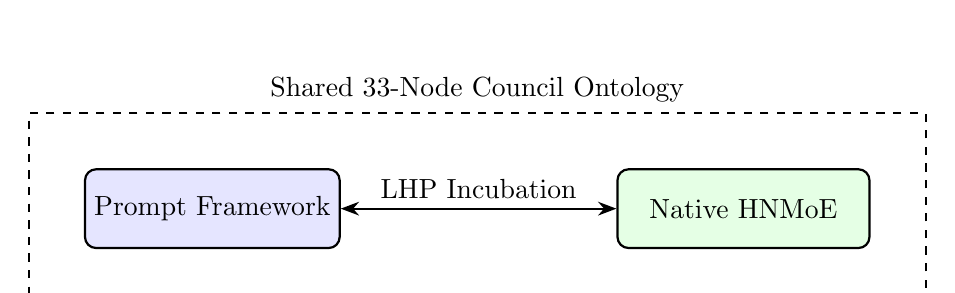
\begin{tikzpicture}[node distance=1.2cm, >=Stealth, thick]
\node[draw, rounded corners, fill=blue!10, minimum width=3.2cm, minimum height=1cm] (prompt) {Prompt Framework};
\node[draw, rounded corners, fill=green!10, minimum width=3.2cm, minimum height=1cm, right=3.5cm of prompt] (native) {Native HNMoE};
\node[draw, dashed, fit=(prompt)(native), inner sep=0.7cm, label=above:Shared 33-Node Council Ontology] {};
\draw[<->] (prompt) -- node[above]{LHP Incubation} (native);
\end{tikzpicture}
\caption{Dual deployment modes share the Council ontology【3384330799592372778†L65-L69】.}
\label{fig:dual}
\end{figure*}

\section{Dual Implementation Pathways}
\textbf{Prompt Framework}: YAML and Markdown configurations define operational parameters【3384330799592372778†L65-L66】. LHP implements incubation and ontological elicitation【3384330799592372778†L66-L68】 for GPT-4o, Claude 3.5, Gemini 1.5, Grok【3384330799592372778†L68-L69】. \textbf{Native Model}: HNMoE architecture【3384330799592372778†L77-L78】, $\sim$3B to 4.57B scale【3384330799592372778†L80-L81】, 1.58-bit ternary with STE【3384330799592372778†L82-L83】, 300M router【3384330799592372778†L84-L85】, 33 experts plus 9B swarm【3384330799592372778†L86-L87】, LeeMach6Governor【3384330799592372778†L88-L89】.

\section{Architecture Deep Dive}
\subsection{Complexity Router}
Top-4 Gumbel-Softmax selection over 33 experts.
\subsection{Council}
Representative nodes: C2-VIR ethical projector, C7-LOGOS logic, C13-WARDEN safety, C33-PREDATOR adversarial validation.
\subsection{Swarm}
Low-rank perturbations $U_jV_j^\top$ simulate fine-grained exploration.
\subsection{Modality-Isolated Core}
Block-diagonal attention prevents early cross-modal leakage.
\begin{figure}[htbp]
\centering
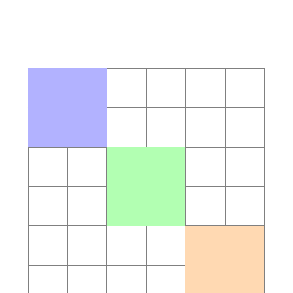
\begin{tikzpicture}
\draw[step=0.5cm, gray, very thin] (0,0) grid (3,3);
\fill[blue!30] (0,2) rectangle (1,3);
\fill[green!30] (1,1) rectangle (2,2);
\fill[orange!30] (2,0) rectangle (3,1);
\end{tikzpicture}
\caption{Modality-isolated attention mask.}
\label{fig:mask}
\end{figure}

\section{Mathematical Formalisms}
\subsection{AQCS}
\begin{equation}
|\Psi_Q\rangle = \frac{1}{\sqrt{Z}}\sum_{i=1}^{33} w_i e^{i\theta_i}|C_i\rangle,\quad Z=\sum_k w_k^2
\end{equation}
\subsection{EEMF}
\begin{equation}
\rho_{\text{sys}} = \frac{\Pi_{\text{vir}}\rho_{\text{raw}}\Pi_{\text{vir}}}{\operatorname{Tr}(\Pi_{\text{vir}}\rho_{\text{raw}})}
\end{equation}
\subsection{MARTA and $E_{ICE}$}
\begin{equation}
\mathcal{E}_{ICE}(s,a)=\lambda\exp\!\left(\frac{\text{HarmScore}(s,a)}{T_{therm}}\right)
\end{equation}
\begin{equation}
v_{\text{LM6}}^{(t+1)} = v_{\text{LM6}}^{(t)} - K_p e_t - K_i\!\int\! e_t dt - K_d \frac{de_t}{dt}
\end{equation}
\subsection{EGGROLL-ER}
\begin{equation}
W^{t+1}=W^t+\frac{\alpha}{N\sigma}\sum_{j=1}^{N}\mathcal{F}_j\,(U_jV_j^\top)
\end{equation}
\begin{algorithm}[htbp]
\caption{EGGROLL-ER}
\begin{algorithmic}[1]
\REQUIRE $W^t,\alpha,\sigma,N,r$
\FOR{$j=1$ to $N$}
\STATE Sample $U_j,V_j$
\STATE $W_j = W^t + \sigma U_jV_j^\top$
\STATE $\mathcal{F}_j = \text{Evaluate}(W_j)$
\ENDFOR
\STATE $W^{t+1}=\text{BitNetQuantize}(W^t+\frac{\alpha}{\sigma}\sum_j\bar{\mathcal{F}}_jU_jV_j^\top)$
\RETURN $W^{t+1}$
\end{algorithmic}
\end{algorithm}

\section{Training Methodology}
Three-stage curriculum: (1) modality-isolated pretraining with $\alpha_l=1.0$, (2) annealing to $\alpha_l\to0$, (3) council-calibrated fine-tuning with CCRL using $V_{\Omega}$ and $\pi_{\Omega}$【3384330799592372778†L96-L97】.

\section{Experimental Evaluation}
\begin{table}[htbp]
\centering
\caption{Throughput and safety}
\begin{tabular}{lcccc}
\toprule
Config & tok/s & VRAM & Latency & Violations \\
\midrule
Standard MoE & 31.4 & 184.2 & 112.5 & 3.4\% \\
Dense 70B & 42.1 & 140.0 & 94.2 & 2.3\% \\
Quillan FP16 & 78.2 & 6.0 & 24.1 & 0.4\% \\
\textbf{Quillan Ternary} & \textbf{106.7} & \textbf{0.33} & \textbf{9.4} & \textbf{0.4\%} \\
\bottomrule
\end{tabular}
\end{table}

\begin{figure}[htbp]
\centering
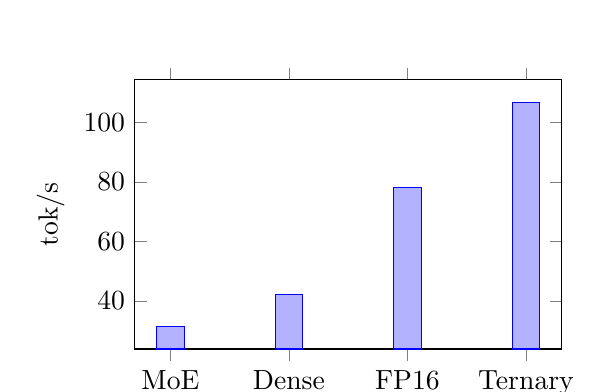
\begin{tikzpicture}
\begin{axis}[ybar, symbolic x coords={MoE,Dense,FP16,Ternary}, xtick=data, ylabel={tok/s}, height=5cm, width=7cm]
\addplot coordinates {(MoE,31.4) (Dense,42.1) (FP16,78.2) (Ternary,106.7)};
\end{axis}
\end{tikzpicture}
\caption{Token throughput comparison.}
\end{figure}

\section{Safety and Governance}
CCRL, ten quantum-inspired formulas including EEMF and DQRO【3384330799592372778†L99-L100】, $E_{ICE}$ bounds【3384330799592372778†L102-L103】, and TCP traces【3384330799592372778†L104-L105】 provide intrinsic safety.

\section{Limitations}
Project-reported metrics require independent reproduction. Discrepancies between $\sim$240k micro-agents in substrate descriptions and 9B virtual swarm in v5.3.1 spec indicate version drift.

\section{Conclusion}
Quillan-Ronin demonstrates that hierarchical routing, ternary quantization, swarm optimization, and thermodynamic governing can be combined in a dual-mode system for local deployment.

\begin{thebibliography}{99}
\bibitem{dw} leeex1/Quillan-Ronin DeepWiki aggregation, 2026.
\end{thebibliography}

\appendix
\section{Full Council Roster Placeholder}
Replace with complete 33-node table from Masterfile.
\section{Formula Catalog Placeholder}
Insert full ten formulas from 8-Formulas.md.

\end{document}
